\section{Introduction}
\label{sec:introduction}

% state the learning objective 
The objective of this laboratory assignment is to study a resistive circuit containing linear components, such as resistors ($R_i$), independent (circle shaped) and dependent (rhombus shaped) voltage ($V$) and current ($I$) sources, as seen in Figure~\ref{fig:esq}. To this end, the currents in every branch and the nodal voltages of the circuit are evaluated, using both the mesh and the nodal methods. For illustration and analysis purposes, the nodes are identified by the red numbers, the elementary meshes by the red subscript letters (in $I_i$) and the arrows point in the conventionalized current way.

In Section \ref{sec:analysis}, a theoretical analysis is presented, using said mesh (in Subsection \ref{subsec:mesh}) and nodal (in Subsection \ref{subsec:node}) methods. In Section~\ref{sec:simulation}, the circuit is analyzed by simulation, using the Ngspice software.
The results are compared in Section \ref{sec:simulation}. The conclusions of this study are outlined in
Section \ref{sec:conclusion}.



\begin{figure}[h] \centering
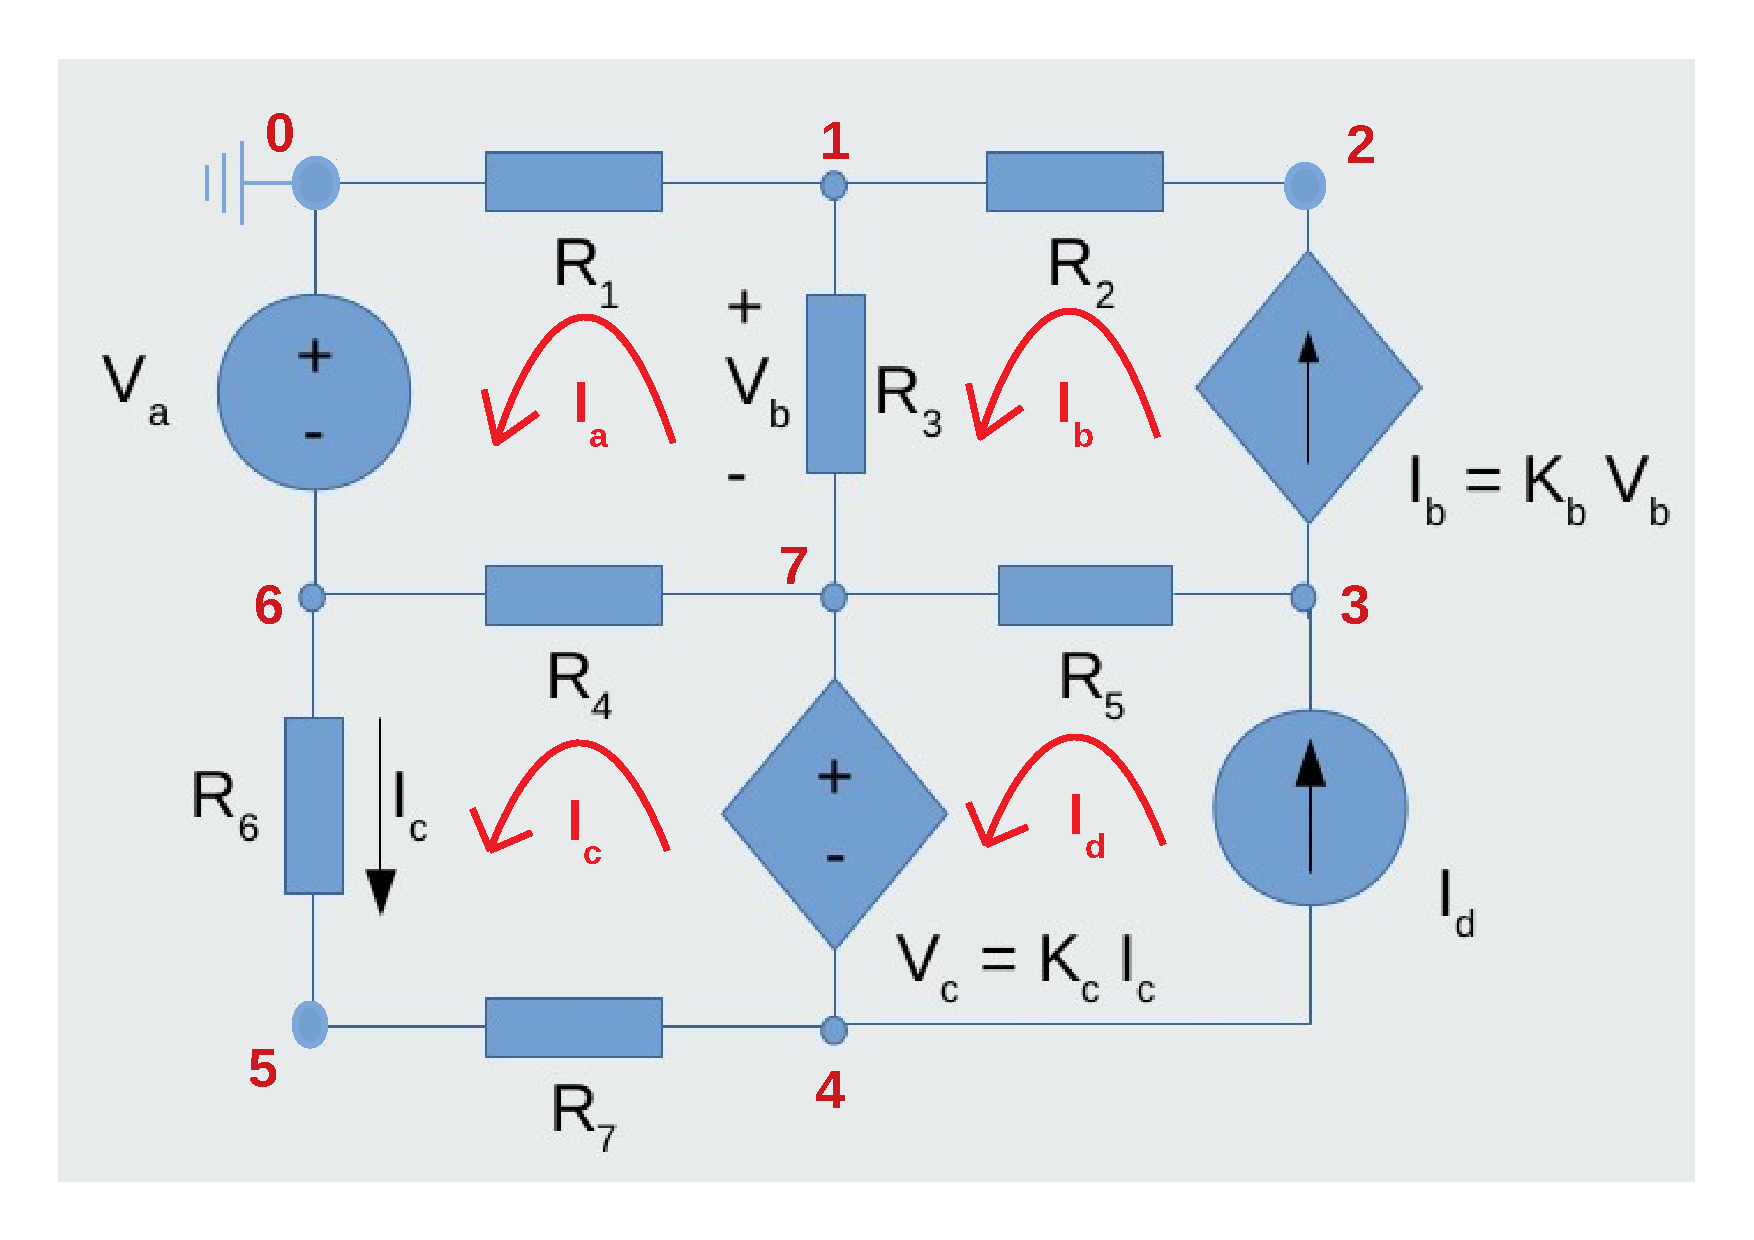
\includegraphics[width=0.8\linewidth]{esq_circ.pdf}
\caption{Resistive circuit.}
\label{fig:esq}
\end{figure}

